% =====================================================================
%  main.tex — master entry point
%  Build: python scripts/build_book.py   (xelatex -> biber -> xelatex x2)
% =====================================================================
\documentclass[11pt,a4paper,oneside,openany]{report}
% =====================================================================
%  preamble.tex — page geometry, fonts, colors, styles and reusable macros
%  Engine: XeLaTeX  |  Language: Hebrew (polyglossia, RTL) + English
% =====================================================================
\usepackage[a4paper,top=2.6cm,bottom=2.4cm,inner=2.3cm,outer=2.3cm,
            headheight=22pt,headsep=12pt,footskip=28pt]{geometry}
\usepackage{fontspec}
\usepackage{amsmath,amssymb}
\usepackage[table]{xcolor}   % table option -> \rowcolor in booktabs tables
\usepackage{graphicx}
\usepackage{tikz}
\usetikzlibrary{shapes.geometric,arrows.meta,positioning,calc,shadows,fit,backgrounds,decorations.pathmorphing}
\usepackage[most]{tcolorbox}
\usepackage{titlesec}
\usepackage{titletoc}
\usepackage{fancyhdr}
\usepackage{booktabs}
\usepackage{tabularx}
\usepackage{array}
\usepackage{enumitem}
\usepackage{caption}
\usepackage{eso-pic}
\usepackage[hidelinks]{hyperref}  % hyperref must precede polyglossia (bidi)
\usepackage{polyglossia}
\setmainlanguage{hebrew}
\setotherlanguage{english}
\usepackage[autostyle=false,style=english]{csquotes} % fixed English quotes in bibliography
% biblatex must load AFTER polyglossia (prototype finding, see docs/PROCESS_LOG.md)
\usepackage[style=numeric,sorting=none,backend=biber,autolang=other]{biblatex}

% ---------- Fonts (Windows system fonts verified in Phase 0) ----------
\setmainfont{David}[Script=Hebrew,Scale=1.12,BoldFont=David Bold]
\setsansfont{Gisha}[Script=Hebrew,BoldFont=Gisha Bold]
\newfontfamily\hebrewfont{David}[Script=Hebrew,Scale=1.12,BoldFont=David Bold]
\newfontfamily\hebrewfontsf{Gisha}[Script=Hebrew,BoldFont=Gisha Bold]
\newfontfamily\englishfont{Arial}[Scale=0.95]
\setmonofont{Courier New}[Scale=0.9]
\newfontfamily\hebrewfonttt{Courier New}[Script=Hebrew,Scale=0.9]

% ---------- Palette ----------
\definecolor{navy}{HTML}{183153}
\definecolor{cream}{HTML}{FFF8ED}
\definecolor{sage}{HTML}{87A98C}
\definecolor{sagedark}{HTML}{4F7656}
\definecolor{coral}{HTML}{E98B73}
\definecolor{coraldark}{HTML}{B5533B}
\definecolor{gold}{HTML}{D8B56A}
\definecolor{golddark}{HTML}{9A7A2E}
\definecolor{charcoal}{HTML}{333333}
\definecolor{alert}{HTML}{B3261E}
\definecolor{paper}{HTML}{FFFCF6}

\pagecolor{paper}
\color{charcoal}
\linespread{1.08}
\setlength{\parindent}{0pt}
\setlength{\parskip}{5pt plus 1pt}
\widowpenalty=10000 \clubpenalty=10000
\emergencystretch=1.5em
% allow line breaks inside long bibliography URLs
\renewcommand*{\bibfont}{\small}
\setcounter{biburlnumpenalty}{100}\setcounter{biburlucpenalty}{200}\setcounter{biburllcpenalty}{100}

% ---------- RTL inside TikZ nodes ----------
% Verified by measurement (Master/work/rtl_tikz_test): TikZ node text is LTR by default under bidi,
% and \setRL has no effect inside nodes. Wrapped nodes (text width): `rtlpar` style.
% Single-line nodes: wrap the text in \RLE{...} (\beginR..\endR misplaced filled labels).
\tikzset{rtlpar/.style={execute at begin node={\begin{RTL}},execute at end node={\end{RTL}}}}

% ---------- Icons (TikZ primitives) ----------
\newcommand{\paw}[1][navy]{%
  \tikz[baseline=-0.6ex,scale=0.11]{%
    \fill[#1] (0,-0.3) ellipse (1.05 and 0.85);
    \fill[#1] (-1.15,0.75) ellipse (0.38 and 0.5);
    \fill[#1] (-0.42,1.35) ellipse (0.38 and 0.5);
    \fill[#1] (0.42,1.35) ellipse (0.38 and 0.5);
    \fill[#1] (1.15,0.75) ellipse (0.38 and 0.5);}}
% Callout title icons — drawn shapes, not punctuation glyphs, so no "!" / "+" character ever
% sits at the start of a Hebrew heading (issue USR-02).
\newcommand{\warnicon}[1][white]{% triangle with an exclamation bar + dot
  \leavevmode\tikz[baseline=-0.585ex,x=0.78ex,y=0.78ex]{%
    \path[use as bounding box] (-1,-0.75) rectangle (1,1.05); % no depth below baseline
    \draw[#1,line width=0.55pt,line join=round,rounded corners=0.3pt] (0,1.05) -- (-1.05,-0.75) -- (1.05,-0.75) -- cycle;
    \fill[#1,rounded corners=0.2pt] (-0.11,0.45) rectangle (0.11,-0.2);
    \fill[#1] (0,-0.45) circle (0.12);}}
\newcommand{\infoicon}[1][white]{% circle with an "i" built from a dot and a bar
  \leavevmode\tikz[baseline=-0.585ex,x=0.78ex,y=0.78ex]{%
    \path[use as bounding box] (-1,-0.75) rectangle (1,1.05); % no depth below baseline
    \draw[#1,line width=0.55pt] (0,0.1) circle (0.95);
    \fill[#1] (0,0.6) circle (0.13);
    \fill[#1,rounded corners=0.2pt] (-0.11,0.3) rectangle (0.11,-0.5);}}
\newcommand{\crossicon}[1][white]{% circled X
  \leavevmode\tikz[baseline=-0.585ex,x=0.78ex,y=0.78ex]{%
    \path[use as bounding box] (-1,-0.75) rectangle (1,1.05); % no depth below baseline
    \draw[#1,line width=0.55pt] (0,0.1) circle (0.95);
    \draw[#1,line width=0.8pt,line cap=round] (-0.42,-0.32) -- (0.42,0.52) (-0.42,0.52) -- (0.42,-0.32);}}
\newcommand{\medicon}[1][white]{% medical cross
  \leavevmode\tikz[baseline=-0.585ex,x=0.78ex,y=0.78ex]{%
    \path[use as bounding box] (-1,-0.75) rectangle (1,1.05); % no depth below baseline
    \fill[#1,rounded corners=0.25pt] (-0.3,-0.75) rectangle (0.3,0.95);
    \fill[#1,rounded corners=0.25pt] (-0.85,-0.2) rectangle (0.85,0.4);}}

% ---------- Chapter openers ----------
\newcommand{\chapsubtitle}{}
\newcommand{\chaptersubtitle}[1]{%
  \vspace*{-6pt}{\sffamily\large\color{coraldark}#1\par}\vspace{8pt}}
\titleformat{\chapter}[block]{\normalfont}{}{0pt}{\chapterbanner}
\titlespacing*{\chapter}{0pt}{-28pt}{12pt}
\newcommand{\chapterbanner}[1]{%
  \begin{tcolorbox}[enhanced,colback=navy,colframe=navy,arc=4mm,
      boxrule=0pt,left=14pt,right=14pt,top=10pt,bottom=12pt,
      overlay={\node[anchor=south west,opacity=0.18] at ([xshift=6pt,yshift=2pt]frame.south west)
                 {\paw[cream]\,\paw[cream]\,\paw[cream]};}]
    {\sffamily\color{gold}\large\bfseries פרק \thechapter\par}\vspace{2pt}
    {\sffamily\color{white}\fontsize{22}{27}\selectfont\bfseries #1\par}
  \end{tcolorbox}}
% Unnumbered chapters (abstract, introduction, bibliography)
\titleformat{name=\chapter,numberless}[block]{\normalfont}{}{0pt}{\plainbanner}
\titlespacing*{name=\chapter,numberless}{0pt}{-28pt}{12pt}
\newcommand{\plainbanner}[1]{%
  {\sffamily\color{navy}\fontsize{22}{27}\selectfont\bfseries #1\par}
  \vspace{2pt}{\color{coral}\rule{0.18\linewidth}{2.2pt}}\par}

\titleformat{\section}{\sffamily\large\bfseries\color{navy}}{\paw[coral]\hspace{6pt}}{0pt}{}
\titlespacing*{\section}{0pt}{11pt}{4pt}
\titleformat{\subsection}{\sffamily\normalsize\bfseries\color{sagedark}}{}{0pt}{}
\titlespacing*{\subsection}{0pt}{7pt}{2pt}
\setcounter{secnumdepth}{0}  % chapters are numbered by the banner; sections stay clean
\setcounter{tocdepth}{1}

% ---------- Table of contents ----------
\titlecontents{chapter}[0pt]{\addvspace{8pt}\sffamily\bfseries\color{navy}}
  {}{}{\titlerule*[0.6pc]{.}\contentspage}
\titlecontents{section}[1.5em]{\addvspace{1pt}\small}
  {}{}{\titlerule*[0.6pc]{.}\contentspage}

% ---------- Headers / footers ----------
\pagestyle{fancy}
\fancyhf{}
\renewcommand{\headrulewidth}{0pt}
\newcommand{\booktitleshort}{המדריך הלא-רשמי לחיים עם כלב בעיר הגדולה}
\fancyhead[R]{\sffamily\footnotesize\color{sagedark}\booktitleshort}
\fancyhead[L]{\sffamily\footnotesize\color{navy}\leftmark}
\fancyfoot[C]{\tikz[baseline=(n.base)]\node[circle,fill=navy,text=white,inner sep=2pt,minimum size=18pt,font=\sffamily\footnotesize\bfseries](n){\thepage};}
\fancypagestyle{plain}{\fancyhf{}\fancyfoot[C]{\tikz[baseline=(n.base)]\node[circle,fill=navy,text=white,inner sep=2pt,minimum size=18pt,font=\sffamily\footnotesize\bfseries](n){\thepage};}}
\renewcommand{\chaptermark}[1]{\markboth{#1}{}}
\renewcommand{\headrule}{{\color{sage}\hrule height 0.6pt}}
\renewcommand{\headrulewidth}{0.6pt}

% ---------- Captions ----------
\DeclareCaptionFont{capnavy}{\color{navy}}
\captionsetup{font={small,sf},labelfont={bf,capnavy},labelsep=colon,justification=centering,skip=6pt}
\captionsetup[table]{position=top}
\renewcommand{\figurename}{איור}
\renewcommand{\tablename}{טבלה}

% ---------- Lists ----------
\setlist{itemsep=1pt,topsep=3pt,parsep=0pt}
\setlist[itemize]{label={\color{coral}\small$\bullet$}}

% ---------- Callout boxes ----------
% ROOT-CAUSE FIX (USR-03, page 9): a tcolorbox title is typeset in vertical mode. When its first
% item is a TikZ picture (paw / icon), the paragraph started left-to-right under bidi, which
% reversed the Hebrew words and left-aligned the title. Starting the paragraph explicitly with
% \leavevmode lets bidi's RTL \everypar apply. Set globally so every current and future box title
% (including inline tcolorboxes such as the Chapter 3 checklist) is covered.
\tcbset{before title={\leavevmode}}
\tcbset{calloutbase/.style={enhanced,breakable,arc=3mm,boxrule=0.8pt,
    left=8pt,right=8pt,top=5pt,bottom=5pt,before skip=8pt,after skip=8pt,
    fonttitle=\sffamily\bfseries\normalsize,coltitle=white,
    attach boxed title to top right={xshift=-10pt,yshift=-8pt},
    boxed title style={arc=2mm,boxrule=0pt}}}
% טיפ חשוב — sage
\newtcolorbox{tipbox}[1][טיפ חשוב]{calloutbase,colback=sage!12!white,colframe=sagedark,
  title={\paw[white]\enspace #1},boxed title style={colback=sagedark}}
% כדאי לדעת — navy
\newtcolorbox{knowbox}[1][כדאי לדעת]{calloutbase,colback=navy!6!white,colframe=navy,
  title={\infoicon\enspace #1},boxed title style={colback=navy}}
% טעות נפוצה — coral
\newtcolorbox{mistakebox}[1][טעות נפוצה]{calloutbase,colback=coral!12!white,colframe=coraldark,
  title={\crossicon\enspace #1},boxed title style={colback=coraldark}}
% שימו לב — gold
\newtcolorbox{notebox}[1][שימו לב]{calloutbase,colback=gold!15!white,colframe=golddark,
  title={\warnicon\enspace #1},boxed title style={colback=golddark}}
% טיפ מהשטח — dashed sage, quote-like
\newtcolorbox{fieldbox}[1][טיפ מהשטח]{enhanced,breakable,arc=3mm,boxrule=0pt,
  colback=cream,left=10pt,right=10pt,top=6pt,bottom=6pt,before skip=8pt,after skip=8pt,
  borderline={1pt}{0pt}{sage,dashed},fontupper=\itshape,
  title={#1},fonttitle=\sffamily\bfseries\small,coltitle=sagedark,
  attach title to upper={\enspace},}
% מידע חירום — strong red frame
\newtcolorbox{emergencybox}[1][מידע חירום — לא לחכות]{enhanced,breakable,arc=2mm,
  boxrule=1.6pt,colframe=alert,colback=alert!5!white,left=10pt,right=10pt,top=6pt,bottom=6pt,
  before skip=8pt,after skip=8pt,
  title={\medicon\enspace #1},fonttitle=\sffamily\bfseries\large,colbacktitle=alert,coltitle=white,
  borderline west={4pt}{0pt}{alert}}

% Small inline LTR helper for English terms / times
\newcommand{\en}[1]{\textenglish{#1}}

% FAQ entries
% same root cause as the box titles: start the paragraph before the TikZ paw
\newcommand{\faq}[1]{\par\addvspace{6pt}{\sffamily\bfseries\color{navy}\leavevmode\paw[coral]\enspace #1\par}\nopagebreak\vspace{1pt}}

\addbibresource{references.bib}
% =====================================================================
%  dog_illustration.tex — ORIGINAL object-based illustration (TikZ primitives)
%  Defines reusable "pics": dog, building, tree, lamp, hydrant, bench
%  and the composed scene \cityScene used on the cover and in Chapter 1.
%  Everything is drawn from ellipses, circles, rounded rectangles and Bézier paths.
% =====================================================================
\definecolor{dogfur}{HTML}{D8B56A}
\definecolor{dogfurdark}{HTML}{A9813A}
\definecolor{dogbelly}{HTML}{F3DFB2}
\definecolor{bldA}{HTML}{24426E}
\definecolor{bldB}{HTML}{2E5486}
\definecolor{bldC}{HTML}{1F3A62}
\definecolor{windowlit}{HTML}{F2D58E}
\definecolor{trunk}{HTML}{7A5A3C}
\definecolor{leaf}{HTML}{87A98C}
\definecolor{leafdark}{HTML}{5F8A66}

\tikzset{
  % ---------------- dog (faces left, origin = middle of body) ----------------
  pics/dog/.style={code={
    % tail (thick rounded Bézier)
    \draw[dogfurdark,line width=4.2pt,line cap=round] (1.45,0.25) .. controls (1.95,0.45) and (2.05,0.95) .. (1.85,1.25);
    % back legs (far side darker, then near side)
    \fill[dogfurdark,rounded corners=2.5pt] (0.95,-0.35) rectangle (1.27,-1.45);
    \fill[dogfurdark,rounded corners=2.5pt] (-0.95,-0.35) rectangle (-0.65,-1.45);
    % body + belly
    \fill[dogfur] (0,0) ellipse (1.55 and 0.68);
    \fill[dogbelly] (-0.15,-0.28) ellipse (0.95 and 0.32);
    % near legs + paws
    \fill[dogfur,rounded corners=2.5pt] (0.55,-0.3) rectangle (0.88,-1.5);
    \fill[dogfur,rounded corners=2.5pt] (-1.3,-0.3) rectangle (-0.98,-1.5);
    \foreach \px in {0.715,-1.14}{\fill[dogbelly] (\px,-1.5) ellipse (0.21 and 0.09);}
    % neck
    \fill[dogfur] (-1.05,0.15) -- (-1.55,1.05) -- (-1.0,1.25) -- (-0.55,0.45) -- cycle;
    % collar + tag
    \fill[coral,rotate around={-58:(-1.18,0.62)}] (-1.48,0.52) rectangle (-0.88,0.72);
    \fill[gold] (-1.32,0.38) circle (0.08);
    % head, snout, nose, tongue
    \fill[dogfur] (-1.45,1.25) circle (0.52);
    \fill[dogbelly] (-1.98,1.08) ellipse (0.48 and 0.3);
    \fill[charcoal] (-2.42,1.16) ellipse (0.12 and 0.09);
    \fill[coral!85!white] (-2.0,0.82) ellipse (0.1 and 0.15);
    \draw[charcoal,line width=0.6pt,line cap=round] (-2.3,1.0) .. controls (-2.15,0.9) .. (-1.95,0.95);
    % eye with highlight
    \fill[charcoal] (-1.62,1.42) circle (0.075);
    \fill[white] (-1.6,1.45) circle (0.025);
    % floppy ear
    \fill[dogfurdark] (-1.3,1.7) .. controls (-0.95,1.65) and (-0.85,1.15) .. (-1.0,0.95)
                       .. controls (-1.15,1.05) and (-1.3,1.3) .. (-1.42,1.55) -- cycle;
  }},
  % ---------------- building: width #1 x height #2 ----------------
  pics/building/.style n args={3}{code={
    \fill[#3] (0,0) rectangle (#1,#2);
    \pgfmathsetmacro{\ncols}{int((#1-0.3)/0.45)}
    \pgfmathsetmacro{\nrows}{int((#2-0.5)/0.55)}
    \foreach \c in {1,...,\ncols}{\foreach \r in {1,...,\nrows}{
      \pgfmathsetmacro{\lit}{mod(\c*7+\r*3,5)<2 ? 1 : 0}
      \ifdim\lit pt>0.5pt \fill[windowlit] ({0.45*\c-0.2},{0.55*\r-0.1}) rectangle +(0.22,0.28);
      \else \fill[white,opacity=0.13] ({0.45*\c-0.2},{0.55*\r-0.1}) rectangle +(0.22,0.28); \fi}}
  }},
  % ---------------- tree ----------------
  pics/tree/.style={code={
    \fill[trunk,rounded corners=1pt] (-0.09,0) rectangle (0.09,0.9);
    \fill[leafdark] (0,1.25) circle (0.55);
    \fill[leaf] (-0.25,1.45) circle (0.42);
    \fill[leaf] (0.28,1.4) circle (0.38);
    \fill[leaf!80!white] (0,1.75) circle (0.33);
  }},
  % ---------------- street lamp ----------------
  pics/lamp/.style={code={
    \draw[charcoal,line width=1.6pt] (0,0) -- (0,2.4) .. controls (0,2.7) .. (0.35,2.7);
    \fill[charcoal] (0.25,2.62) rectangle (0.55,2.72);
    \fill[gold,opacity=0.9] (0.4,2.58) circle (0.09);
    \fill[gold,opacity=0.18] (0.4,2.4) circle (0.42);
  }},
  % ---------------- fire hydrant ----------------
  pics/hydrant/.style={code={
    \fill[coraldark,rounded corners=1.5pt] (-0.16,0) rectangle (0.16,0.5);
    \fill[coraldark] (0,0.5) circle (0.17);
    \fill[coral] (-0.26,0.25) rectangle (0.26,0.36);
    \fill[coral] (-0.22,0) rectangle (0.22,0.06);
  }},
  % ---------------- bench ----------------
  pics/bench/.style={code={
    \fill[trunk] (0,0.35) rectangle (1.1,0.43);
    \fill[trunk] (0,0.55) rectangle (1.1,0.62);
    \draw[charcoal,line width=1.2pt] (0.12,0) -- (0.12,0.62) (0.98,0) -- (0.98,0.62);
  }},
}

% ---------------- cat (sitting, faces right) ----------------
\tikzset{pics/cat/.style={code={
    \draw[charcoal,line width=3pt,line cap=round] (-0.45,-0.55) .. controls (-1.0,-0.6) and (-1.0,0.1) .. (-0.75,0.3);
    \fill[charcoal] (0,-0.1) ellipse (0.55 and 0.62);
    \fill[charcoal] (0.15,0.75) circle (0.38);
    \fill[charcoal] (-0.12,0.95) -- (-0.05,1.32) -- (0.18,1.07) -- cycle;
    \fill[charcoal] (0.18,1.07) -- (0.42,1.3) -- (0.48,0.92) -- cycle;
    \fill[gold] (0.05,0.8) ellipse (0.07 and 0.09);
    \fill[gold] (0.32,0.8) ellipse (0.07 and 0.09);
    \fill[charcoal!40!black] (0.05,0.8) ellipse (0.02 and 0.07);
    \fill[charcoal!40!black] (0.32,0.8) ellipse (0.02 and 0.07);
    \fill[coral!80!white] (0.19,0.66) circle (0.035);
    \fill[charcoal] (-0.25,-0.72) ellipse (0.18 and 0.08);
    \fill[charcoal] (0.25,-0.72) ellipse (0.18 and 0.08);
}}}

% ---------------- elevator scene: three dogs and one unimpressed cat ----------------
\newcommand{\elevatorScene}{%
\begin{tikzpicture}[scale=0.85]
  % shaft wall + open doors
  \fill[cream!70!sage] (-0.6,-0.3) rectangle (9.6,5.0);
  \fill[white] (0,0) rectangle (9,4.4);
  \fill[sage!25!white] (0,0) rectangle (9,0.35);
  \draw[navy,line width=2pt,rounded corners=2pt] (0,0) rectangle (9,4.4);
  \fill[navy!15!white] (-0.45,0) rectangle (0,4.4);
  \fill[navy!15!white] (9,0) rectangle (9.45,4.4);
  % floor indicator & buttons
  \fill[navy,rounded corners=2pt] (3.9,4.55) rectangle (5.1,4.95);
  \node[text=gold,font=\sffamily\bfseries\small] at (4.5,4.75) {\textenglish{7}};
  \foreach \y in {1.9,2.25,2.6}{\fill[gold] (8.6,\y) circle (0.08);}
  % characters
  \pic[scale=0.42] at (1.9,1.05) {dog};
  \pic[scale=0.62] at (4.4,1.35) {dog};
  \pic[scale=0.32] at (6.4,0.85) {dog};
  \pic[scale=0.75] at (8.0,0.95) {cat};
  % speech-like thought from the cat
  \node[draw=charcoal,fill=white,rounded corners=4pt,font=\sffamily\scriptsize,inner sep=3pt]
       at (7.1,3.55) {\RLE{זאת הייתה מעלית שלי.}};
  \draw[charcoal] (7.75,3.3) -- (7.95,2.4);
\end{tikzpicture}}

% ---------------- composed scene: city street with a dog on a walk ----------------
% #1 = overall scale
\newcommand{\cityScene}[1][1]{%
\begin{tikzpicture}[scale=#1,every node/.style={transform shape}]
  % sky band + sun
  \fill[cream] (-0.2,-0.2) rectangle (14.2,6.6);
  \fill[gold!55!white] (11.6,5.3) circle (0.75);
  \fill[gold!30!white,opacity=0.6] (11.6,5.3) circle (1.05);
  % skyline
  \pic at (0,1.2) {building={2.0}{4.6}{bldC}};
  \pic at (2.2,1.2) {building={1.6}{3.3}{bldB}};
  \pic at (3.95,1.2) {building={2.3}{5.2}{bldA}};
  \pic at (6.45,1.2) {building={1.5}{2.8}{bldB}};
  \pic at (8.1,1.2) {building={2.2}{4.1}{bldC}};
  \pic at (10.5,1.2) {building={1.6}{3.0}{bldA}};
  \pic at (12.3,1.2) {building={1.8}{4.4}{bldB}};
  % sidewalk & curb
  \fill[sage!35!cream] (-0.2,0.0) rectangle (14.2,1.2);
  \fill[sage!60!white] (-0.2,1.12) rectangle (14.2,1.25);
  \foreach \x in {0.6,2.6,...,13}{\draw[sage!70!white,line width=0.6pt] (\x,0.05) -- (\x+0.5,1.1);}
  % street furniture
  \pic at (1.3,1.2) {tree};
  \pic at (6.9,1.2) {tree};
  \pic at (13.1,1.2) {tree};
  \pic at (4.4,1.2) {lamp};
  \pic at (10.0,1.25) {hydrant};
  \pic at (11.3,1.2) {bench};
  % leash path to an off-frame hand (top-right), then the dog
  \draw[navy,line width=1.1pt] (7.55,2.55) .. controls (8.6,3.3) and (9.2,3.9) .. (9.6,4.6);
  \fill[navy] (9.6,4.6) circle (0.11);
  \pic[scale=0.8] at (8.5,2.4) {dog};
  % small paw-print trail
  \foreach \x/\y in {10.6/0.55,11.3/0.75,12.0/0.5,12.7/0.72}{
     \fill[navy,opacity=0.25] (\x,\y) ellipse (0.09 and 0.07);}
\end{tikzpicture}}

\graphicspath{{../figures/generated/}}

\gappto\captionshebrew{%
  \renewcommand{\contentsname}{תוכן עניינים}%
  \renewcommand{\figurename}{איור}%
  \renewcommand{\tablename}{טבלה}%
  \renewcommand{\bibname}{מקורות}}

\hypersetup{pdftitle={המדריך הלא-רשמי לחיים עם כלב בעיר הגדולה},
            pdfsubject={בין פחמימות לטיולי לילה: המדריך השלם לבעלי כלבים עירוניים},
            pdfcreator={XeLaTeX + Claude Code (master / detector / fixer)}}

\begin{document}

% ---------------- Front matter ----------------
% =====================================================================
%  cover.tex — full-bleed cover. Illustration = \cityScene (figures/tikz/dog_illustration.tex)
% =====================================================================
\thispagestyle{empty}
\begin{tikzpicture}[remember picture,overlay,hebpar/.style={rtlpar}]
  % navy background with a subtle diagonal sheen
  \fill[navy] (current page.south west) rectangle (current page.north east);
  \fill[white,opacity=0.035] ([yshift=-2cm]current page.north west) -- ([yshift=-9cm]current page.north east)
        -- (current page.north east) -- (current page.north west) -- cycle;
  % top label
  \node[anchor=north east,font=\sffamily\large,text=gold] at ([xshift=-2.3cm,yshift=-2.2cm]current page.north east)
       {\RLE{\paw[gold]\enspace מדריך מאויר לבעלי כלבים עירוניים}};
  % title block
  \node[hebpar,anchor=north east,align=right,text width=16.5cm,font=\sffamily\bfseries,text=white]
       at ([xshift=-2.3cm,yshift=-3.4cm]current page.north east)
       {\fontsize{40}{46}\selectfont המדריך הלא-רשמי\\[2pt]
        \fontsize{30}{38}\selectfont לחיים עם כלב בעיר הגדולה};
  \fill[coral] ([xshift=-2.3cm,yshift=-7.25cm]current page.north east) rectangle ++(-3.2cm,-0.14cm);
  \node[hebpar,anchor=north east,align=right,text width=16cm,font=\sffamily\Large,text=cream]
       at ([xshift=-2.3cm,yshift=-7.75cm]current page.north east)
       {בין פחמימות לטיולי לילה:\\ המדריך השלם לבעלי כלבים עירוניים};
  % illustration panel
  \node[anchor=center,inner sep=0pt] (scene) at ([yshift=-2.6cm]current page.center)
       {\scalebox{1.18}{\begin{tikzpicture}\clip[rounded corners=8mm] (-0.2,-0.2) rectangle (14.2,6.6);
        \node[inner sep=0pt,anchor=south west] at (-0.2,-0.2){\cityScene[1]};\end{tikzpicture}}};
  % footer: authors placeholders (to be supplied by the students — not invented)
  \node[hebpar,anchor=south east,align=right,text width=12cm,font=\sffamily,text=cream]
       at ([xshift=-2.3cm,yshift=2.2cm]current page.south east)
       {\large מחברות ומחברים: [שמות המחברים — יושלם]\\[3pt]
        \normalsize קוד קבוצה: [XXXXXXXX] \quad·\quad 2026};
  \node[anchor=south west,font=\sffamily\small,text=sage] at ([xshift=2.3cm,yshift=2.2cm]current page.south west)
       {\textenglish{Typeset with XeLaTeX · Illustrated with TikZ \& Python}};
\end{tikzpicture}
\clearpage

% =====================================================================
%  abstract.tex — תקציר
% =====================================================================
\chapter*{תקציר}
\addcontentsline{toc}{chapter}{תקציר}
\thispagestyle{plain}

כלב בעיר הגדולה חי בעולם שלא תוכנן בשבילו: מעליות צפופות, צופרים, אופניים חשמליים,
מדרכות שמתחממות בקיץ ושכנים שלא תמיד מתלהבים לפגוש לשון רטובה בשבע בבוקר. לבעלים, העיר מוסיפה
לוח זמנים לחוץ, דירה קטנה והחלטות יומיומיות קטנות שמצטברות לאיכות החיים של הכלב.

\textbf{המדריך הלא-רשמי לחיים עם כלב בעיר הגדולה} מרכז את ההחלטות האלה בארבעה פרקים קצרים ומעשיים.
\textbf{הפרק הראשון} עוסק בפסיכולוגיה של הכלב העירוני: איך לזהות סימני נוחות ואי-נוחות, ומדוע חיזוק
חיובי ושגרה צפויה עוזרים לכלב להתמודד עם גירויים. \textbf{הפרק השני} מלמד למפות את השכונה
מנקודת המבט של הכלב, כולל צל, מים, חום המדרכה ותנועה. \textbf{הפרק השלישי} עוסק בלוגיסטיקה:
מה לוקחים לטיול, איך מתכננים את היום ואיך מחשבים את זמן ההליכה היומי. \textbf{הפרק הרביעי} הוא
מדריך הישרדות בפורמט של שאלות ותשובות, ובו תרשים החלטה לרגע שבו הכלב מרים משהו חשוד מהרצפה.

המדריך כתוב בגובה העיניים ועם לא מעט הומור, אבל ההמלצות בו נשענות על מקורות וטרינריים ומקצועיים
המופיעים ברשימת המקורות. הוא אינו מחליף ייעוץ וטרינרי: כל כלב שונה, וכשיש ספק, הווטרינר
הוא הכתובת.

\vfill
\begin{knowbox}[למי המדריך מיועד]
לבעלי כלבים בפעם הראשונה, לדיירי דירות ולמי שמנסים לשלב עבודה, חיים חברתיים וטיולים.
המדריך מתאים לכלבים קטנים, בינוניים וגדולים, ומזכיר לאורך הדרך שגיל, בריאות ומזג משנים את התמונה.
\end{knowbox}
\vfill
\clearpage


\tableofcontents
\thispagestyle{plain}
\clearpage

% =====================================================================
%  introduction.tex — מבוא
% =====================================================================
\chapter*{מבוא: עיר אחת, שני מינים}
\addcontentsline{toc}{chapter}{מבוא}
\markboth{מבוא}{}
\thispagestyle{plain}

השעה \en{06:52}. אתם עדיין בפיג\gr מה, הקפה עוד לא מוכן, ומישהו עומד ליד הדלת ומסתכל עליכם במבט שאומר
"זה הרגע הכי חשוב בחיים שלי". מבחינתו זה באמת כך: הטיול של הבוקר הוא העיתון, הרשת החברתית
וחדר הכושר שלו, הכול ביחד.

החיים עם כלב בעיר הם שותפות בין שני מינים שחווים את אותו רחוב בצורה שונה לגמרי. אתם רואים
מעבר חצייה, אוטובוס ובית קפה. הכלב מריח את ההיסטוריה של כל עמוד חשמל, שומע את האופניים החשמליים
הרבה לפני שאתם שמים לב אליהם, ומבין מצוין שהשקית המרשרשת בכיס שלכם עשויה להכיל משהו טעים.

\secnotoc{איך לקרוא את המדריך}
כל פרק עומד בפני עצמו, אפשר לקפוץ ישר למה שבוער. לאורך הדרך תפגשו תיבות מידע בצבעים שונים,
וכל צבע מסמן סוג אחר של מידע:

\begin{itemize}
  \item \textcolor{sagedark}{\textbf{טיפ חשוב:}} המלצה מעשית שכדאי ליישם כבר בטיול הבא.
  \item \textcolor{navy}{\textbf{כדאי לדעת:}} רקע מקצועי קצר שעוזר להבין \emph{למה}.
  \item \textcolor{coraldark}{\textbf{טעות נפוצה:}} דברים שכולנו עשינו לפחות פעם אחת.
  \item \textcolor{golddark}{\textbf{שימו לב:}} עניינים של בטיחות.
  \item \textcolor{sagedark}{\textbf{טיפ מהשטח:}} הניסיון המצטבר של בעלי כלבים עירוניים.
  \item \textcolor{alert}{\textbf{מידע חירום:}} מצבים שבהם לא מחכים, אלא פונים לווטרינר.
\end{itemize}

\begin{notebox}[הבהרה חשובה]
המדריך נועד להעשרה ולהתמצאות כללית בלבד. הוא לא מאבחן, לא מטפל ולא מחליף ייעוץ אישי אצל
וטרינר או מאלף מוסמך. גם ההמלצות לגבי משכי טיול הן דוגמאות ולא הוראות: גיל, גזע, בריאות ומזג
של כל כלב משנים את התמונה.
\end{notebox}

\secnotoc{מה בפנים}
\textbf{פרק~1} עוסק בראש של הכלב, \textbf{פרק~2} במפה של השכונה, \textbf{פרק~3} בתיק ובשעון,
ו\textbf{פרק~4} ברגעים שבהם משהו משתבש. בסוף המדריך תמצאו מילון מונחים, דף מסכם למקרר,
רשימת מקורות ועמוד שמתאר איך הספר נבנה: במערכת הסדר \en{LaTeX}, בקוד \en{Python} ובשפת השרטוט
\en{TikZ}, ובעזרת שלושה סוכני \en{Claude Code} שעבדו כצוות.

\begin{fieldbox}
הכלב שלכם לא קרא את המדריך הזה. הוא מומחה לעצמו, ולכן כל טיפ כאן שווה בדיוק כמו המידה שבה הוא
מתאים לכלב הספציפי שעומד עכשיו ליד הדלת.
\end{fieldbox}
\clearpage


% ---------------- Chapters ----------------
% =====================================================================
%  chapter01_psychology.tex — הפסיכולוגיה של הכלב העירוני
% =====================================================================
\chapter{הפסיכולוגיה של הכלב העירוני}
\chaptersubtitle{איך לשרוד מעלית עם שלושה כלבים וחתול}

\section{העיר מגובה חצי מטר}
נסו לרדת לרגע לגובה של כלב בינוני. המכוניות נראות פתאום כמו קירות נעים, הצופר של האוטובוס
מגיע בדיוק בגובה האוזניים, ורגליים של זרים חולפות במרחק נגיעה. מעליכם מתנהלת שיחה שאתם לא
מבינים, ומתחתיכם מדרכה שמספרת סיפור ריחני על כל מי שעבר בה היום.

לחלק מהכלבים זה גן עדן. אחרים פשוט צריכים יותר זמן להתרגל, ויש כלבים שהעומס הזה מתיש אותם.
אין כאן "נכון" אחד: גנטיקה, ניסיון מוקדם, גיל ובריאות משפיעים על האופן שבו כל כלב חווה את
הרחוב. המשימה שלנו היא ללמוד לקרוא את הכלב \emph{שלנו}, לא את הכלב הממוצע.

\section{רשימת הגירויים העירונית}
מכוניות וצפירות, אופניים וקורקינטים חשמליים שמופיעים בלי רעש, מעליות שנסגרות בחבטה, ילדים
שרצים לחבק, כלבים אחרים מעבר לכביש ושקית פלאפל שמישהו שכח על הספסל. כל אחד מהגירויים האלה
לבדו הוא עניין קטן. כשהם מצטברים בטיול אחד, חלק מהכלבים מגיעים לעומס חושי: הם מתקשים להקשיב,
מושכים, נובחים או "נתקעים" במקום.

\begin{knowbox}
התנהגות "קשה" ברחוב היא לפעמים לא חוסר חינוך אלא סימן לכך שהכלב מוצף. ארגוני רווחת בעלי חיים
ממליצים ללמוד את שפת הגוף של הכלב כדי לזהות לחץ מוקדם, לפני שהוא מסלים~\cite{rspca-behaviour}.
\end{knowbox}

\section{שפת הגוף: מה הכלב מנסה להגיד}
כלבים "מדברים" בעיקר בגוף. הטבלה הקטנה שבהמשך היא נקודת פתיחה בלבד: תמיד מסתכלים על \emph{כל}
הגוף ועל ההקשר, ולא על סימן בודד. גם זנב מכשכש לא אומר בהכרח שהכלב שמח: לפעמים כך נראית
דווקא התרגשות מתוחה.

\begin{tcbraster}[raster columns=3,raster equal height,raster column skip=6pt,
   raster before skip=6pt,raster after skip=8pt,
   raster every box/.append style={before upper={\raggedright}}] % ragged end side (DET-1-08)
  \begin{tcolorbox}[enhanced,colback=sage!14!white,colframe=sagedark,arc=2mm,boxrule=0.8pt,
     title={\sffamily\bfseries רגוע ונינוח},colbacktitle=sagedark,fontupper=\small,left=4pt,right=4pt]
    גוף רפוי, פה פתוח מעט, תנועות "גליות", זנב בגובה טבעי, מבט רך.
  \end{tcolorbox}
  \begin{tcolorbox}[enhanced,colback=gold!16!white,colframe=golddark,arc=2mm,boxrule=0.8pt,
     title={\sffamily\bfseries סקרן או נרגש},colbacktitle=golddark,fontupper=\small,left=4pt,right=4pt]
    אוזניים קדימה, גוף נוטה לעבר הגירוי, ריחרוח ממוקד. התרגשות יכולה להיראות כמו קפיצות ומשיכה.
  \end{tcolorbox}
  \begin{tcolorbox}[enhanced,colback=coral!14!white,colframe=coraldark,arc=2mm,boxrule=0.8pt,
     title={\sffamily\bfseries לחוץ או מפחד},colbacktitle=coraldark,fontupper=\small,left=4pt,right=4pt]
    זנב מקופל, אוזניים לאחור, ליקוק שפתיים, פיהוק "לא במקום", לובן עין גלוי, קפיאה או ניסיון לברוח~\cite{rspca-behaviour,aspcapro-body}.
  \end{tcolorbox}
\end{tcbraster}

ההבדל בין התרגשות לפחד לא תמיד ברור, וזה בסדר. אם אתם לא בטוחים, תנו לכלב יותר מרחק מהגירוי
ובדקו אם הגוף שלו משתחרר. כלב שנרגע כשמתרחקים כנראה היה בלחץ.

\section{חיזוק חיובי ושגרה צפויה}
הדרך היעילה ביותר לעזור לכלב עם העיר היא ללמד אותו שדברים מפחידים מנבאים דברים טובים: חטיף
כשהאוטובוס עובר, שבח כשהוא מסתכל עליכם במקום על הכלב שממול. איגוד הווטרינרים האמריקאי לרפואה
התנהגותית (\en{AVSAB}) ממליץ על אימון מבוסס תגמול ומתנגד לשימוש בשיטות ענישה~\cite{avsab2021}, וסקירת
מחקר וסקר בקרב בעלי כלבים מצאו ששיטות אימון מבוססות ענישה או הפחדה קשורות לסיכון גבוה יותר
לבעיות התנהגות ולפגיעה ברווחה~\cite{ziv2017,hiby2004}.

שגרה עוזרת לא פחות. כלב שיודע מתי יוצאים, באיזה מסלול ומה קורה בסוף, מתמודד בקלות רבה יותר
עם ההפתעות שהעיר תמיד מספקת.

\section{מעלית: שלושה כלבים, חתול אחד וארבע קומות של מתח}

\begin{figure}[h]
  \centering
  \elevatorScene
  \caption{"מעלית לקומה 7". איור מקורי שנבנה בקוד \en{TikZ} מצורות גאומטריות (כלב, חתול, מעלית).}
  \label{fig:elevator}
\end{figure}

קומה 3. הדלת נפתחת. בפנים: רקסי, בורדר קולי עם תוכניות; פיצי, צ\gr יוואווה עם דעות; ומיסטר ביג,
דני ענק שמנסה להיראות קטן. בפינה יושב החתול של הקומה השביעית, שרכב במעלית הזאת עוד לפני
שמישהו מהנוכחים נולד. כולם מסתכלים על כולם. אף אחד לא נושם.

הנה איך זה \emph{לא} נגמר בבלגן:

\begin{tipbox}[כללי המעלית]
\begin{itemize}
  \item \textbf{שואלים לפני שנכנסים.} "זה בסדר אם אצטרף עם הכלב?" זאת לא חולשה, זה נימוס.
  \item \textbf{רצועה קצרה, לא מתוחה.} הכלב צמוד אליכם, והרצועה רפויה ולא נכרכת סביב רגליים.
  \item \textbf{פנים אל הדלת, גב אל הקיר.} מקטינים מבטים ישירים בין בעלי החיים.
  \item \textbf{מחכים למעלית הבאה} כשהכלב שלכם, או של מישהו אחר, נראה לחוץ. ההמתנה קצרה, התקרית
        ארוכה.
  \item \textbf{מתגמלים שקט.} חטיף קטן על ישיבה רגועה הופך את המעלית ממלכודת לחוויה טובה.
\end{itemize}
\end{tipbox}

\section{מפגשים עם כלבים אחרים ומרחב אישי}
לא כל כלב רוצה להכיר כל כלב, בדיוק כמו שלא כל אדם רוצה לדבר עם כל מי שעומד איתו בתור. מפגש
"אף מול אף" על מדרכה צרה, ברצועה, הוא מצב רגיש במיוחד: לאף אחד מהכלבים אין לאן לזוז.
שאלו את הבעלים לפני שמתקרבים, אפשרו לכלבים להיפגש בקשת ולא חזיתית, וסיימו את המפגש אחרי כמה
שניות, כשכולם עוד נהנים.

\begin{mistakebox}
"הוא ידידותי!" זה משפט נחמד, אבל הוא מתאר רק את הכלב \emph{שלכם}. ייתכן שהכלב השני חולה, מבוגר,
בשיקום או פשוט לא במצב רוח. מרחב אישי הוא זכות גם בעולם של ארבע רגליים.
\end{mistakebox}

\begin{fieldbox}
"שיטת הקשת": כשכלב מתקרב מולכם ואתם לא בטוחים, חצו לצד השני או עשו עיקוף קטן. הכלב שלכם
יקבל מרחק, ואתם תקבלו עוד שנייה לחשוב.
\end{fieldbox}

\section{גור בעיר: לאט, ובקצב של הכלב}
גורים לומדים על העולם במהירות, והחוויות של החודשים הראשונים משפיעות על האופן שבו יתמודדו
עם העיר בהמשך. איגוד הווטרינרים האמריקאי לרפואה התנהגותית ממליץ על חשיפה מוקדמת, מבוקרת
וחיובית לסביבות, לאנשים ולגירויים, בתיאום עם הווטרינר לגבי מצב החיסונים~\cite{avsab-puppy}.
המילה החשובה כאן היא \emph{הדרגתית:} לא "להטביע" את הגור ברעש של מרכז העיר, אלא לבנות סולם.

\begin{figure}[h]
  \centering
  \resizebox{0.97\linewidth}{!}{% =====================================================================
%  exposure_ladder.tex — "סולם החשיפה": gradual exposure to city stimuli (Chapter 1)
%  Five rising steps drawn from rounded rectangles; progression reads right -> left (Hebrew).
%  RTL: wrapped node text uses the `rtlpar` style, single-line labels use \RLE{} (see preamble).
% =====================================================================
\begin{tikzpicture}[
    font=\sffamily\small,
    ladderstep/.style={rtlpar,draw=none,rounded corners=2.5mm,align=center,text width=2.55cm,
                 inner sep=4pt,anchor=south,text=white},
    num/.style={circle,fill=white,text=navy,font=\sffamily\scriptsize\bfseries,inner sep=1.2pt,minimum size=13pt}
  ]
  % ground line
  \draw[sage!60!white,line width=1.2pt] (-0.4,0) -- (15.6,0);
  % steps: \i = position, colour mixes sage -> coral as difficulty rises
  \foreach \i/\head/\body in {
      1/צפייה מרחוק/מספסל ברחוב שקט,
      2/רחוב שקט/הליכה קצרה ומעט אנשים,
      3/רעשים מוכרים/אוטובוס עובר במרחק,
      4/מקום הומה/כמה דקות ליד בית קפה,
      5/מעלית ושכנים/נסיעה קצרה וחטיף בסוף}{
    \pgfmathsetmacro{\x}{14.0-3.15*(\i-1)}
    \pgfmathsetmacro{\h}{1.15+0.42*(\i-1)}
    \pgfmathsetmacro{\mix}{100-25*(\i-1)}
    \fill[sagedark!\mix!coraldark,rounded corners=2.5mm] (\x-1.42,0) rectangle (\x+1.42,\h);
    \node[ladderstep] at (\x,0.08) {\textbf{\head}\\[1pt]{\footnotesize \body}};
    \node[num] at (\x+1.3,\h) {\i};
  }
  % progression arrow (right -> left) above the steps
  \draw[-{Stealth[length=7pt]},navy,line width=1pt] (15.3,3.35) -- (-0.2,3.35);
  \node[fill=paper,inner sep=2pt,font=\sffamily\footnotesize\bfseries,text=navy] at (7.6,3.35)
       {\RLE{מתקדמים שלב רק כשהכלב רגוע בשלב הקודם}};
\end{tikzpicture}
}
  \caption{סולם החשיפה: דוגמה לחשיפה הדרגתית לגירויים עירוניים. כל שלב נמשך כמה ימים או שבועות,
  לפי תגובת הגור. איור מקורי בקוד \en{TikZ}.}
  \label{fig:ladder}
\end{figure}

בכל שלב מחפשים את אותם סימני נינוחות מהטבלה שלמעלה. אם הגור קופא, מנסה לברוח או מסרב לחטיף
שהוא בדרך כלל אוהב, זה סימן לחזור שלב אחד אחורה ולהגדיל את המרחק. הצלחה נמדדת בגור רגוע, לא
במספר הגירויים שהספקתם לסמן ביום אחד.

\section{לבד בבית: הדירה כשאתם בעבודה}
כלבים עירוניים רבים מבלים חלק מהיום לבד. חלקם ישנים בשלווה עד שאתם חוזרים, ואחרים מתקשים: נביחות
ממושכות, הרס ליד הדלת, ריור או צרכים בבית. חשוב לזכור שזו לא "נקמה": התנהגויות כאלה הן לרוב
סימן למצוקה כשהכלב נשאר לבד, ואפשר למנוע אותן ולטפל בהן~\cite{rspca-separation}.

\begin{tipbox}[לפני שיוצאים מהבית]
\begin{itemize}
  \item \textbf{טיול ממוקד לפני היציאה}, עם הרבה זמן ריחרוח, ולא רק "סיבוב להוריד".
  \item \textbf{העסקה:} צעצוע שאפשר למלא באוכל, משחק חיפוש או לעיסה מתאימה לגודל הכלב.
  \item \textbf{פרידה וחזרה שגרתיות:} בלי טקס ארוך ובלי התרגשות, כדי שהיציאה תהיה עניין רגיל.
  \item \textbf{תרגול הדרגתי:} מתחילים מהיעדרויות של דקות ספורות ומאריכים לאט.
\end{itemize}
\end{tipbox}

\begin{knowbox}[מתי לבקש עזרה]
אם השכנים מדווחים על נביחות ממושכות, או שהכלב פוגע בעצמו או בדלת, אל תחכו שזה "יעבור". פנו
לווטרינר כדי לשלול סיבה רפואית, ולאחר מכן למאלף או ליועץ התנהגות שעובד בשיטות מבוססות תגמול
\cite{avsab2021,rspca-separation}.
\end{knowbox}

% =====================================================================
%  chapter02_city_mapping.tex — מיפוי שטח
% =====================================================================
\chapter{מיפוי שטח}
\chaptersubtitle{הגיאוגרפיה של גינות כלבים ופינות הצל הנכונות}

\section{המפה שבראש של הכלב}
לכם יש \en{Waze}. לכלב יש מפה אחרת לגמרי: איפה העץ שכולם מסמנים, איפה הברזייה, איפה החתול
שיושב על הגדר ואיפה המדרכה שבקיץ שורפת את הכפות. בעלי כלבים ותיקים מפתחים עם הזמן מפה כפולה,
שמשלבת את מה שנוח לבני אדם עם מה שבטוח ומעניין לכלב. הפרק הזה עוזר לבנות אותה בכוונה ולא רק
בדרך של ניסוי וטעייה.

\begin{figure}[h]
  \centering
  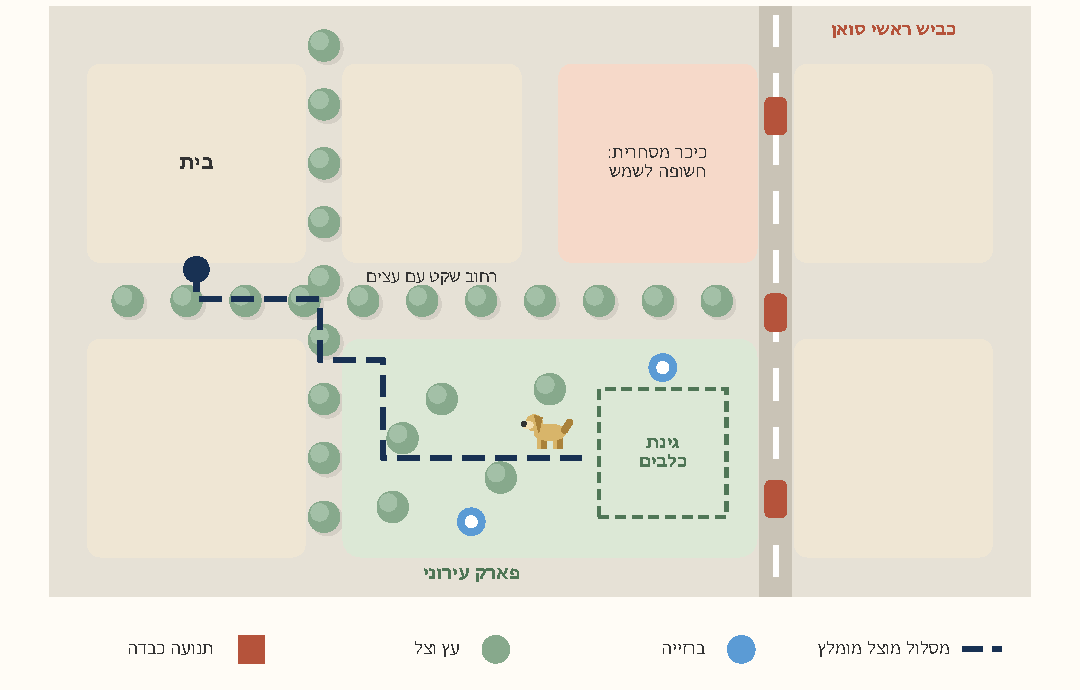
\includegraphics[width=0.86\linewidth]{original_neighborhood_map.pdf}
  \caption{מפת שכונה קונספטואלית: מסלול מוצל מהבית לגינת הכלבים, הרחק מהכביש הסואן ומהכיכר
  החשופה. איור מקורי שנוצר בקוד \en{Python} (\en{matplotlib}) מצורות גאומטריות. השכונה בדיונית.}
  \label{fig:map}
\end{figure}

\section{חמש שאלות לפני שבוחרים מסלול}
\begin{enumerate}[label=\textbf{\arabic*.},leftmargin=*]
  \item \textbf{צל:} כמה מהמסלול עובר מתחת לעצים או בצד המוצל של הרחוב, בשעה שבה אתם יוצאים?
  \item \textbf{מים:} יש ברזייה בדרך? אם לא, אתם המים. על זה בפרק 3.
  \item \textbf{משטח:} אספלט, אבן, דשא או חול? משטחים כהים וחשופים מתחממים מאוד בשמש.
  \item \textbf{תנועה:} כמה מעברי חציה, כמה כבישים ראשיים, וכמה אופניים וקורקינטים במדרכה?
  \item \textbf{עומס:} כמה אנשים, כלבים ורעש יש במסלול בשעה הזאת? לכלב רגיש, שקט שווה יותר מקיצור דרך.
\end{enumerate}

\section{מדרכה חמה, כפות רגישות}
בימים חמים האספלט יכול להתחמם הרבה יותר מהאוויר, ואיגוד הווטרינרים האמריקאי (\en{AVMA}) מזהיר
שמשטחים חמים עלולים לגרום לכוויות בכפות. הוא ממליץ להגביל פעילות בימים חמים, לדאוג לצל ולמים
ולהעדיף את השעות הקרירות של היום \cite{avma-warm}. מחקר על כלבים בבריטניה מצא שפעילות גופנית
היא אחד הגורמים השכיחים למכת חום בכלבים, ושהסיכון גבוה יותר בכלבים ברכיצפליים (בעלי אף קצר), בכלבים
כבדים ובכלבים מבוגרים \cite{hall2020}.

\begin{notebox}
בדיקה מעשית שנפוצה בקרב בעלי כלבים: הניחו את גב כף היד על המדרכה לכמה שניות. אם לא נוח לכם
להשאיר אותה שם, כנראה שזה חם מדי גם לכפות. זו בדיקה גסה, לא מדידה. בימים חמים במיוחד
עדיף לקצר, ללכת על דשא או בצל, או לדחות את הטיול לשעה קרירה יותר.
\end{notebox}

\section{גינת כלבים או רחוב שקט?}
גינת כלבים היא מקום נהדר לכלב חברותי שאוהב לרוץ, אבל היא לא חובה, ולא כל כלב נהנה בה.
כשבודקים גינה, כדאי להסתכל על הגדר והשער הכפול, על הצל ועל המים, על מספר הכלבים בשעה
שבה אתם מגיעים ועל ההתנהגות של הבעלים: האם מישהו בכלל מסתכל על הכלב שלו?

\begin{table}[h]
\centering
\caption{השוואה בין סביבות הליכה עירוניות (הערכה כללית, משתנה משכונה לשכונה)}
\label{tab:areas}
\renewcommand{\arraystretch}{1.35}
\small
\begin{tabularx}{\linewidth}{>{\sffamily\bfseries\color{navy}}p{2.1cm} X X X}
\toprule
{\sffamily\bfseries סוג אזור} & {\sffamily\bfseries יתרונות} & {\sffamily\bfseries אתגרים} & {\sffamily\bfseries מתי כדאי לבחור בו} \\
\midrule
פארק עירוני & שטח פתוח, דשא, עצים ולרוב גם ברזיות & רוכבי אופניים, פיקניקים ושאריות אוכל & טיול ארוך בבוקר או לפני השקיעה \\
\rowcolor{sage!10}
רחוב שקט & מעט רעש ותנועה, קל לשמור על קשב & לעיתים מעט צל, מכוניות חונות שמסתירות שדה ראייה & טיול קצר, כלב רגיש או גור בתחילת הדרך \\
גינת כלבים & ריצה חופשית במרחב מגודר ומפגש חברתי & צפיפות, מתחים בין כלבים, צל ומים לא תמיד זמינים & כלב חברותי, בשעות פחות עמוסות \\
\rowcolor{sage!10}
טיילת & מסלול ארוך ורציף, נוף ורוח & חשיפה לשמש, הרבה אנשים, אופניים וקורקינטים & ערב או בוקר מוקדם, כשהמשטח קריר \\
אזור מסחרי & הרגלה לגירויים, סידורים בדרך & רעש, צפיפות, אוכל על הרצפה ומדרכות חמות & אימון קצר ומבוקר, לא כטיול עיקרי \\
\bottomrule
\end{tabularx}
\end{table}

\section{לחיות ביחד במרחב הציבורי}
העיר שייכת לכולם, גם למי שמפחד מכלבים. בישראל, החוק להסדרת הפיקוח על כלבים קובע כללים להחזקת
כלבים במרחב הציבורי, ובהם חובת רצועה \cite{il-doglaw2002}. בנוסף, לרשויות המקומיות יש חוקי עזר
משלהן, למשל לגבי איסוף צואה ואזורים שבהם מותר לשחרר כלבים. לכן כדאי לבדוק באתר העירייה שלכם מה
חל בשכונה. אוספים כל צואה, מקצרים את הרצועה ליד ילדים, רוכבים ושולחנות של בתי קפה, וזוכרים
שהכלב שלכם הוא השגריר של כל בעלי הכלבים ברחוב.

\begin{fieldbox}
בנו לעצמכם שלושה מסלולים קבועים: \textbf{קצר} לימים עמוסים, \textbf{מוצל} לימים חמים
ו\textbf{ארוך} לסופי שבוע. כשמזג האוויר או מצב הרוח משתנים, לא צריך לתכנן מחדש, רק לבחור.
\end{fieldbox}

% =====================================================================
%  chapter03_logistics.tex — לוגיסטיקה ואופרציות
% =====================================================================
\chapter{לוגיסטיקה ואופרציות}
\chaptersubtitle{איך לארגן את התיק לטיול של חמש דקות שנגמר בשעה}

\section{האנטומיה של ״אני רק יוצא לשנייה״}
כל בעל כלב מכיר את זה: יצאתם ״רק להוריד אותו״, בכפכפים ובלי טלפון, ואז הכלב מצא חבר, השכן
מצא נושא לשיחה והשמש החליטה לצאת במלוא העוצמה. הטיול של חמש דקות נמשך שעה, ואתם בלי מים ובלי
שקית שנייה. הפתרון הוא לא לצאת פחות, אלא להתארגן פעם אחת ולהפסיק לחשוב על זה.

\section{הערכה הבסיסית}
\begin{tcolorbox}[enhanced,colback=white,colframe=navy,arc=3mm,boxrule=0.8pt,
   title={\sffamily\bfseries\paw[white]\enspace רשימת ציוד קבועה ליד הדלת},colbacktitle=navy,
   left=8pt,right=8pt]
\begin{itemize}[label={\color{sagedark}$\square$}]
  \item \textbf{רצועה וקולר או רתמה תקינים}, עם תג ובו מספר טלפון עדכני. בישראל החוק מחייב גם
        סימון בשבב אלקטרוני, רישוי וחיסון נגד כלבת \cite{il-doglaw2002}.
  \item \textbf{שקיות לאיסוף צואה}: תמיד אחת יותר ממה שנראה לכם הגיוני.
  \item \textbf{מים וכלי שתייה מתקפל}, במיוחד בימים חמים ובמסלולים בלי ברזייה \cite{avma-warm}.
  \item \textbf{חטיפים קטנים} לתגמול על התנהגות רגועה (ראו פרק 1).
  \item \textbf{טלפון טעון} ומספר הווטרינר ומוקד החירום הקרוב שמורים בו מראש.
  \item \textbf{לפי מזג האוויר}: מעיל לכלב קטן או קצר-פרווה בחורף, ופנס או אפוד מחזיר-אור בלילה.
\end{itemize}
\end{tcolorbox}

\begin{fieldbox}
קנו שני עותקים מכל דבר קטן: שקיות, כלי שתייה וחטיפים. סט אחד גר קבוע בתיק הטיולים, והסט השני
במגירה ליד הדלת. ככה לא ״שואלים״ ציוד מתיק לתיק, ולא נשארים בלי.
\end{fieldbox}

\section{המתמטיקה של יום עירוני}
כדי לתכנן יום עמוס, כדאי לדעת כמה זמן הטיולים לוקחים בפועל. מספר הטיולים ביום יסומן באות $n$,
ומשך הטיול מספר $i$ (בדקות) יסומן $t_i$. זמן הטיול היומי הכולל הוא:

\begin{equation}
  T_{\text{daily}} \;=\; \sum_{i=1}^{n} t_i
  \label{eq:daily}
\end{equation}

\textbf{דוגמה היפותטית:} נניח ארבעה טיולים: 20 דקות בבוקר, 15 בצהריים, 35 בערב ועשר דקות לפני השינה.
אז
\[
  T_{\text{daily}} = 20 + 15 + 35 + 10 = 80 \ \text{min}.
\]
כלומר, כשעה ועשרים דקות ביום, ועוד ״מקדם הפתעות״ של מפגשים, ריחות ושכנים. בפועל, כדאי לשריין
ביומן קצת יותר ממה שהנוסחה אומרת.

\begin{figure}[h]
  \centering
  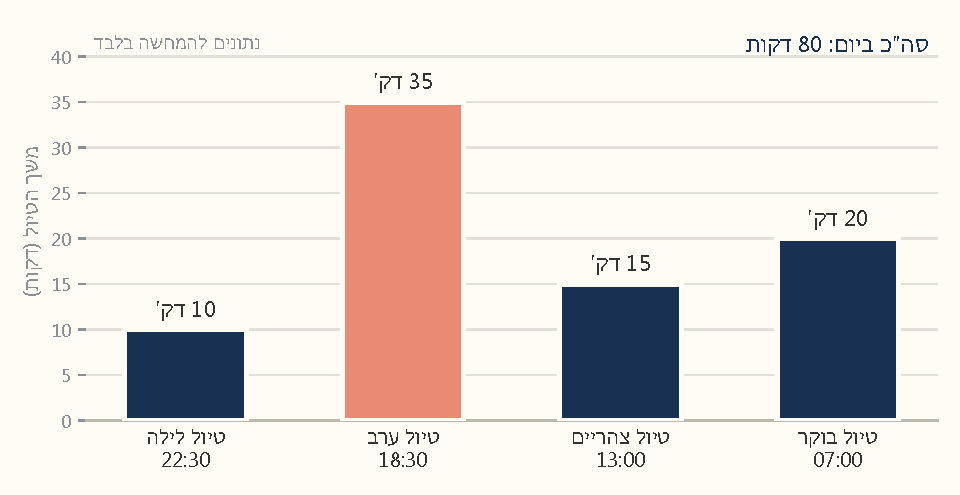
\includegraphics[width=0.82\linewidth]{activity_graph.pdf}
  \caption{חלוקת זמן הטיולים לאורך יום עירוני לדוגמה. הגרף נוצר בקוד \en{Python} (\en{matplotlib})
  מהנתונים של הדוגמה שלמעלה. \textbf{הנתונים להמחשה בלבד} ואינם המלצה וטרינרית.}
  \label{fig:graph}
\end{figure}

\begin{knowbox}
אין ״מספר דקות נכון״ אחד לכל הכלבים. גור, כלב צעיר ואנרגטי, כלב מבוגר וכלב עם בעיה רפואית צריכים
דברים שונים מאוד, וגם מזג האוויר משנה את התמונה. את הכמות והעצימות המתאימות לכלב שלכם כדאי לקבוע
יחד עם הווטרינר.
\end{knowbox}

\section{לתכנן סביב עבודה, חיים ובלת״מים}
\begin{itemize}
  \item \textbf{עוגנים קבועים:} טיול בוקר וטיול ערב בשעות דומות בכל יום יוצרים שגרה צפויה.
  \item \textbf{תוכנית ב׳ לצהריים:} שכנה, בן משפחה או מוליך כלבים, ומספר טלפון שמור מראש.
  \item \textbf{״מקדם עיכוב״:} הוסיפו ליומן כרבע שעה רזרבה סביב כל טיול. מה שלא נוצל הוא בונוס.
  \item \textbf{ימים חמים:} מקדימים את הבוקר, מאחרים את הערב ומקצרים את הצהריים
        (ראו פרק 2 ומקור \cite{avma-warm}).
\end{itemize}

\section{שבוע לדוגמה}
השגרה היומית מתחברת לשבוע. הטבלה הבאה היא דוגמה היפותטית למשק בית עם שני אנשים עובדים וכלב
בוגר ובריא. היא לא מתכון: המטרה היא להראות איך מחלקים אחריות כך שאף טיול לא ״נופל בין הכיסאות״.

\begin{table}[h]
\centering
\caption{שבוע לדוגמה: מי מוציא את הכלב ומתי (נתונים להמחשה בלבד)}
\label{tab:week}
\renewcommand{\arraystretch}{1.3}
\small
\begin{tabularx}{\linewidth}{>{\sffamily\bfseries\color{navy}}p{1.9cm} X X X}
\toprule
{\sffamily\bfseries יום} & {\sffamily\bfseries בוקר} & {\sffamily\bfseries צהריים} & {\sffamily\bfseries ערב ולילה} \\
\midrule
ראשון–רביעי & א׳: טיול רגיל & שכנה או מוליך כלבים & ב׳: טיול ארוך, ואחר כך יציאה קצרה \\
\rowcolor{sage!10}
חמישי & ב׳: טיול רגיל & א׳ עובד מהבית & טיול משותף לגינת הכלבים \\
שישי & טיול ארוך בפארק & יציאה קצרה & א׳: טיול רגיל \\
\rowcolor{sage!10}
שבת & טיול רגוע עם הרבה ריחרוח & מנוחה, משחקי חיפוש בבית & ב׳: טיול רגיל \\
\bottomrule
\end{tabularx}
\end{table}

\begin{fieldbox}
תלו את הטבלה על המקרר או שתפו אותה ביומן משותף. כשמשהו משתנה, מעדכנים במקום אחד, וכל מי
שמעורב בטיפול בכלב רואה את אותה תמונה.
\end{fieldbox}

\section{תיק חירום קטן}
מלבד תיק הטיולים היומי, כדאי להכין בבית תיק קטן שמוכן ליום שבו משהו משתבש: נסיעה דחופה
לווטרינר, הפסקת חשמל ארוכה או פינוי זמני מהבית.
\begin{itemize}
  \item צילום של פנקס החיסונים ומספר השבב, גם בטלפון וגם על נייר.
  \item רצועה וקולר רזרביים, עם תג זיהוי מעודכן.
  \item מזון ומים לכמה ימים, וכלי האכלה מתקפל.
  \item תרופות קבועות, אם יש כאלה, לפי הנחיות הווטרינר.
  \item ערכת עזרה ראשונה לבעלי חיים, שאת תכולתה כדאי לתאם עם הווטרינר.
  \item מגבת, שקיות ותמונה עדכנית של הכלב, למקרה שיאבד.
\end{itemize}

\begin{mistakebox}
לצאת ״על הדרך״ לסידורים עם כלב שלא רגיל לכך: תור בדואר, חנות צפופה ומדרכה רותחת. לכלב זה
עומס חושי, ולכם זה תור שנמשך כפליים. עדיף טיול קצר וממוקד, ואת הסידורים לעשות אחר כך.
\end{mistakebox}

% =====================================================================
%  chapter04_survival.tex — מדריך הישרדות: שאלות נפוצות ותקלות נפוצות
% =====================================================================
\chapter{מדריך הישרדות}
\chaptersubtitle{שאלות נפוצות ותקלות נפוצות}

הפרק הזה בנוי כמו מוקד שירות: שאלה, תשובה קצרה וצעד הבא. החלק הראשון עוסק בתקלות
יומיומיות, והחלק השני במצבים שבהם צריך לחשוב על פנייה לווטרינר.

\section{תקלות יומיומיות}

\faq{הכלב מסרב להיכנס למעלית. מה עושים?}
לא גוררים. מתרגלים כשאין לחץ: עומדים ליד המעלית ומתגמלים, אחר כך נכנסים ויוצאים בלי לנסוע, ורק
אז נוסעים קומה אחת. בינתיים, אם אפשר, משתמשים במדרגות. אם הסירוב מופיע פתאום אצל כלב שתמיד
נכנס בשמחה, כדאי לחשוב גם על כאב או שינוי בריאותי ולהתייעץ עם הווטרינר.

\faq{הכלב נלחץ ליד תנועה סואנת}
מגדילים מרחק: הולכים בצד הפנימי של המדרכה, בוחרים רחובות שקטים יותר (פרק 2) ומתגמלים כל מבט
רגוע לעבר הכביש. מתחילים מגירוי חלש ורחוק, ומתקרבים בהדרגה לאורך ימים ושבועות. זה עובד טוב יותר
מאשר ״לחשוף עד שיתרגל״.

\faq{הכלב מגיב בעוצמה לכלבים זרים}
יוצרים מרחק ושוברים קו ראייה: עוברים מאחורי רכב חונה, חוצים את הכביש או מסתובבים. לא צועקים
ולא מושכים בחוזקה, כי שני הדברים מעלים את המתח. אם התגובות חוזרות, כדאי לפנות למאלף שעובד
בשיטות מבוססות תגמול \cite{avsab2021}.

\faq{לוח הזמנים התפרק: ישיבה התארכה, רכבת התעכבה}
בשביל זה בדיוק קיימת ״תוכנית ב׳״ מפרק 3: איש קשר שיכול להוציא את הכלב, וחלון זמן גמיש. כשחוזרים
מאוחר, טיול קצר ורגוע עדיף על ניסיון ״לפצות״ בריצה ארוכה בחושך.

\faq{הכלב מוצף בסביבה עמוסה}
יוצאים מהסביבה העמוסה לפינה שקטה, נותנים לכלב לרחרח (ריחרוח מרגיע כלבים רבים) ומסיימים את הטיול
מוקדם. בפעם הבאה מגיעים לאותו מקום בשעה פחות עמוסה ולזמן קצר יותר.

\faq{שכחתי שקית, מים או חטיפים}
שקית: בקשו מבעלי כלבים אחרים, רובם ישמחו לעזור. מים: קצרו את הטיול, בחרו מסלול מוצל ועם
ברזייה. בפעם הבאה תעזור ״ערכת הכפילות״ מפרק 3.

\section{כשזה כבר לא יומיומי}

\faq{מזג האוויר התחמם מאוד באמצע הטיול}
עוברים לצל, מאטים ומציעים מים. מקצרים את הטיול וחוזרים הביתה בדרך המוצלת ביותר. כלבים עם אף
קצר, כלבים כבדים ומבוגרים נמצאים בסיכון גבוה יותר למכת חום \cite{hall2020}. איגוד הווטרינרים
האמריקאי מונה בין סימני האזהרה התנשפות חזקה, ריור מרובה, חולשה או חוסר יציבות, הקאה, לשון כהה
במיוחד, פרכוסים ואובדן הכרה \cite{avma-warm}. אם מופיעים סימנים כאלה, פונים מיד לווטרינר.

\faq{הכלב הרים או בלע משהו מהרחוב}
שאריות פיתה, עצם מבושלת, מסטיק או תרופה שמישהו איבד. ברחוב העירוני יש הכול. חלק ממזונות האדם
מסוכנים לכלבים, למשל שוקולד, ענבים וצימוקים, ומוצרים שמכילים קסיליטול כמו חלק מסוגי המסטיקים
ללא סוכר \cite{aspca-foods}. כשיש חשד להרעלה, הנחיית ארגון \en{ASPCA} היא לפנות מיד לווטרינר או
למוקד הרעלות לבעלי חיים \cite{aspca-apcc}. התרשים הבא מסכם את סדר הפעולות.

\begin{figure}[h]
  \centering
  % =====================================================================
%  eight_block_diagram.tex — decision workflow with EXACTLY EIGHT blocks
%  "מה עושים כשהכלב מרים משהו חשוד מהרצפה?"
%  Blocks = the eight \node commands with style `blk`, `startblk`, `endblk` or `decision`
%  (B1..B8). Edge labels are plain text annotations on arrows, not blocks.
%  Layout: row 1 reads right->left (Hebrew order), row 2 left->right, row 3 bottom.
% =====================================================================
\begin{tikzpicture}[
    font=\sffamily\small,
    node distance=1.0cm,
    base/.style={rtlpar,draw,line width=0.9pt,align=center,text width=3.6cm,minimum height=1.25cm,inner sep=4pt},
    blk/.style={base,rounded corners=3mm,fill=white,draw=navy},
    startblk/.style={base,rounded corners=6mm,fill=sage!30!white,draw=sagedark},
    endblk/.style={base,rounded corners=6mm,fill=gold!30!white,draw=golddark},
    urgent/.style={base,rounded corners=3mm,fill=alert!9!white,draw=alert,line width=1.4pt},
    decision/.style={rtlpar,draw=coraldark,fill=coral!18!white,line width=0.9pt,diamond,aspect=1.9,
                     align=center,text width=2.9cm,inner sep=0pt},
    arr/.style={-{Stealth[length=7pt]},line width=1.0pt,draw=navy},
    lbl/.style={font=\sffamily\footnotesize\bfseries,text=coraldark,fill=paper,inner sep=1.5pt},
    num/.style={circle,fill=navy,text=white,font=\sffamily\scriptsize\bfseries,inner sep=1.2pt,minimum size=13pt}
  ]
  % ---- Row 1 (right -> left) ----
  \node[startblk] (B1) at (12.4,0)  {הכלב הרים או לעס משהו חשוד מהרצפה};
  \node[blk]      (B2) at (7.2,0)   {הרחיקו אותו בעדינות מהמקום, אם זה בטוח};
  \node[blk]      (B3) at (2.0,0)   {נסו לזהות מה זה היה: צלמו או שמרו אריזה ושארית};
  % ---- Row 2 ----
  % "ייתכן" = is it POSSIBLE: an unsure answer is a "yes" (safety-first branching)
  \node[decision] (B4) at (2.0,-3.0) {ייתכן שמשהו נבלע, או שיש סימני מצוקה?};
  \node[urgent]   (B6) at (7.2,-3.0) {פנו מיד לווטרינר או למוקד חירום. אל תגרמו להקאה בעצמכם};
  \node[blk]      (B7) at (12.4,-3.0){פעלו בדיוק לפי הנחיות הווטרינר};
  % ---- Row 3 ----
  \node[blk]      (B5) at (2.0,-6.0) {בוודאות לא נבלע דבר: עקבו אחר הכלב בשעות הקרובות};
  \node[endblk]   (B8) at (12.4,-6.0){תעדו את האירוע ושפרו את המניעה בטיול הבא};

  % ---- step numbers (badges, not blocks) ----
  \foreach \b/\n in {B1/1,B2/2,B3/3,B5/5,B6/6,B7/7,B8/8}{\node[num] at (\b.north east) {\n};}
  % west vertex: the 3->4 arrowhead at the top vertex stays visible (DET-1-07)
  \node[num] at (B4.west) {4};

  % ---- arrows ----
  \draw[arr] (B1) -- (B2);
  \draw[arr] (B2) -- (B3);
  \draw[arr] (B3) -- (B4);
  \draw[arr] (B4) -- node[lbl,above=3pt,pos=0.45] {\RLE{כן}} (B6);
  \draw[arr] (B6) -- (B7);
  \draw[arr] (B4) -- node[lbl,left=2pt] {\RLE{לא, בוודאות}} (B5); % left side: clear of badge 5 and connector (DET-1-07)
  \draw[arr] (B5.east) -- node[lbl,above=1pt] {\RLE{הכול תקין}} (B8.west);
  \draw[arr] ([xshift=-0.4cm]B5.north east) |- ([yshift=-0.45cm]B6.south) -- (B6.south);
  \node[lbl,anchor=north] at ([yshift=-0.5cm,xshift=0.3cm]B6.south) {\RLE{הופיע סימן חריג}};
  \draw[arr] (B7) -- (B8);
\end{tikzpicture}

  \caption{מה עושים כשהכלב מרים משהו חשוד מהרצפה? תרשים זרימה בן שמונה שלבים (נבנה בקוד \en{TikZ}).
  התרשים נועד להתמצאות ואינו מחליף ייעוץ וטרינרי.}
  \label{fig:flow}
\end{figure}

\begin{emergencybox}
\begin{itemize}
  \item \textbf{אל תגרמו להקאה} ואל תיתנו תרופה או ״תרופת סבתא״ בלי הנחיה מפורשת של וטרינר.
  \item \textbf{קשיי נשימה, קריסה, פרכוסים, חולשה פתאומית או הקאות חוזרות}: נוסעים מיד למרפאה
        או לבית חולים וטרינרי, ומתקשרים בדרך.
  \item \textbf{מה לקחת:} את האריזה, שארית החומר או תמונה שלו, ומידע על הזמן המשוער שבו זה קרה.
  \item \textbf{מספרי חירום שמורים מראש:} הווטרינר הקבוע ומוקד החירום הקרוב, כבר עכשיו ולא ברגע האמת.
\end{itemize}
\end{emergencybox}


% ---------------- Back matter ----------------
% =====================================================================
%  acknowledgments.tex — מקורות (עמוד 19) + על הספר: קרדיטים ואיך נבנה הספר (עמוד 20)
% =====================================================================
\chapter*{מקורות}
\addcontentsline{toc}{chapter}{מקורות}
\markboth{מקורות}{}
\thispagestyle{plain}

הטענות העובדתיות במדריך מבוססות על המקורות שלהלן. הבדיקה של כל טענה מול המקור שלה מתועדת
במסמך ביקורת המקורות (\en{Source Audit}) שבמאגר הפרויקט.

\begin{english}
\printbibliography[heading=none]
\end{english}
\clearpage

% ---------------------------------------------------------------------
\chapter*{על הספר}
\addcontentsline{toc}{chapter}{על הספר}
\markboth{על הספר}{}
\thispagestyle{plain}

\secnotoc{קרדיטים לחומרים חזותיים}
כל האיורים, הגרפים והתרשימים בספר מקוריים ונוצרו בקוד. קבצי המקור שלהם נמצאים בתיקייה \en{figures}
שבמאגר הפרויקט, וכולם נוצרים מחדש בפקודת בנייה אחת.
\begin{itemize}
  \item \textbf{איור השער ואיור \ref{fig:elevator}}: איורים שנבנו בקוד \en{TikZ} מצורות גאומטריות.
  \item \textbf{איור \ref{fig:ladder}}: סולם החשיפה, תרשים בקוד \en{TikZ}.
  \item \textbf{איור \ref{fig:map}}: מפה קונספטואלית שנוצרה בקוד \en{Python}.
  \item \textbf{איור \ref{fig:graph}}: גרף שנוצר בקוד \en{Python} מנתוני המחשה.
  \item \textbf{איור \ref{fig:flow}}: תרשים זרימה בן שמונה שלבים בקוד \en{TikZ}.
\end{itemize}

\secnotoc{איך נבנה הספר}
הספר נכתב ונבנה כפרויקט \en{Vibe Coding}, כלומר פיתוח בהנחיה בשפה טבעית בעזרת \en{Claude Code}.
הטקסט נכתב בעזרת \en{XeLaTeX} עם \en{polyglossia}, לתמיכה בעברית ובכיווניות מימין לשמאל, והגרפים
והאיורים נוצרו בקוד \en{Python} ובשפת השרטוט \en{TikZ}.

תהליך העבודה תוכנן סביב שלושה סוכנים בעלי תפקידים נפרדים, שעובדים על אותו מאגר קבצים:

\begin{center}
\begin{tikzpicture}[font=\sffamily\small,
    agent/.style={rtlpar,draw,rounded corners=3mm,line width=1pt,align=center,text width=3.3cm,
                  minimum height=1.5cm,inner sep=4pt},
    arr/.style={-{Stealth[length=6pt]},line width=0.9pt,draw=navy},
    lbl/.style={font=\sffamily\scriptsize,text=charcoal,fill=paper,inner sep=1.5pt}]
  \node[agent,fill=navy!8!white,draw=navy]          (M) at (11,0)  {\textbf{\en{Master}}\\ כתיבה, עיצוב וניהול};
  \node[agent,fill=coral!14!white,draw=coraldark]   (D) at (5.5,0) {\textbf{\en{Detector}}\\ בדיקת איכות עצמאית};
  \node[agent,fill=sage!20!white,draw=sagedark]     (F) at (0,0)   {\textbf{\en{Fixer}}\\ אימות מקורות ותיקונים};
  \draw[arr] ([yshift=5pt]M.west) -- node[lbl,above=2pt]{\RLE{בקשת בדיקה}} ([yshift=5pt]D.east);
  \draw[arr] ([yshift=-5pt]D.east) -- node[lbl,below=2pt]{\RLE{דוח ליקויים}} ([yshift=-5pt]M.west);
  \draw[arr] (M.north) -- ++(0,0.55) -| node[lbl,pos=0.25,above=1pt]{\RLE{בקשת תיקון ואימות מקורות}} (F.north);
  \draw[arr] (F.south) -- ++(0,-0.55) -| node[lbl,pos=0.25,below=1pt]{\RLE{בקשה לבדיקה חוזרת}} (D.south);
\end{tikzpicture}
\end{center}

\en{Master} כותב ומעצב את הספר ומחליט על קבלת השינויים, \en{Detector} בודק באופן עצמאי את השפה,
הפריסה והעמידה בדרישות, ו\en{Fixer} מאמת את המקורות ומתקן ליקויים שאושרו. מצב הביצוע בפועל של
כל שלב, כולל אילו בדיקות כבר הושלמו, מתועד ביומני התהליך ובדוחות הבדיקה שבמאגר הפרויקט.
בינה מלאכותית שימשה ככלי עבודה, והאחריות לתוכן נשארת של המחברות.

\vfill
\begin{knowbox}[מגישות]
ליה פורת ורוני ברק \enspace·\enspace קוד קבוצה: \en{liyaroni-ex2} \enspace·\enspace 2026
\end{knowbox}


\end{document}
